%%%%%%%%%%%%%%%%%%%%%%%%%%%%%%%%
% Compile with
% pdflatex --shell-escape -synctex=1 -interaction=nonstopmode rasterGrid.tex
% to convert it to png use:
% convert -density 300 -transparent white "\image.pdf" "\image.png"},
%%%%%%%%%%%%%%%%%%%%%%%%%%%%%%%%

\documentclass{standalone}

\usepackage[utf8]{inputenc}
\usepackage{tkz-fct}
\renewcommand{\familydefault}{\sfdefault}
\usepackage[scaled=1]{helvet}
\usepackage[helvet]{sfmath}
\everymath={\sf}
\usepackage{pagecolor}
\usetikzlibrary{calc,arrows,intersections,angles,quotes,patterns, backgrounds, shapes.misc}

\definecolor{AFLight}{HTML}{5CE0E6}
\definecolor{AFMiddle}{HTML}{51ADE5}
\definecolor{AFDark}{HTML}{0E4160}
\definecolor{AFOppo}{HTML}{FFB150}


\begin{document}

\tikzset{
   every node/.style={scale=1.3},
   >=stealth
}

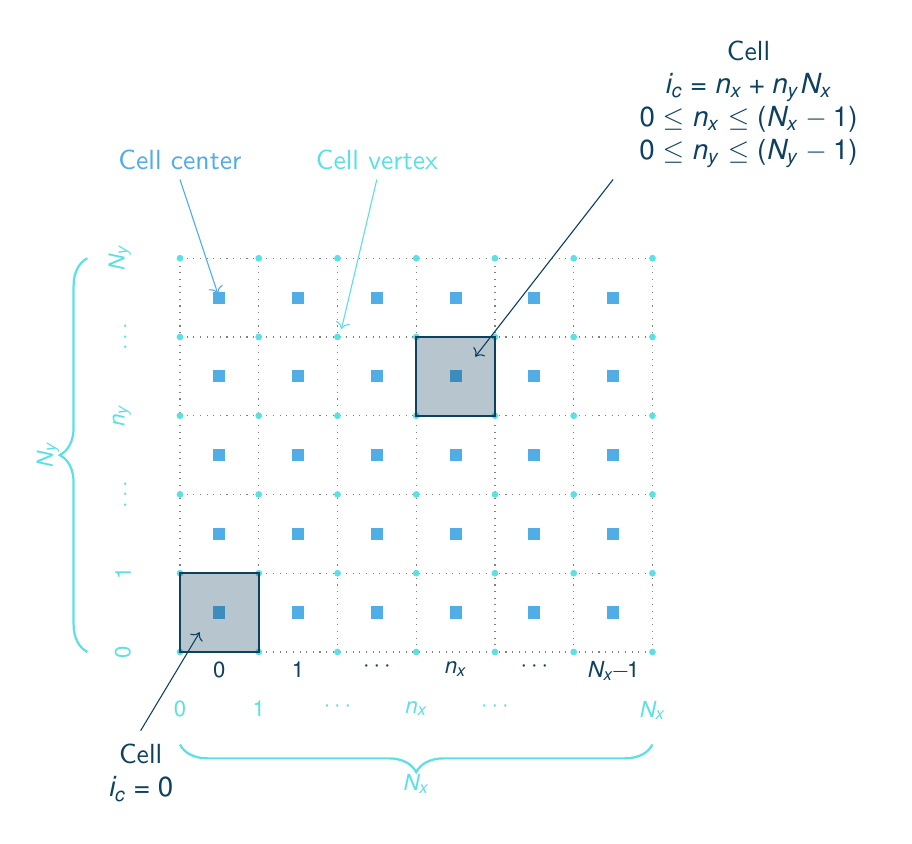
\begin{tikzpicture}[
    scale=1
 ]
\def\xMin{0}
\def\xMinSec{1}
\def\yMin{0}
\def\yMinSec{1}
\def\xMax{6}
\def\yMax{5}

\def\xxMin{0.5}
\def\xxMinSec{1.5}
\def\yyMin{0.5}
\def\yyMinSec{1.5}
\def\xxMax{5.5}
\def\yyMax{4.5}
    \foreach \i in {\xMin,\xMinSec,...,\xMax} {
        \draw [thin, dotted, gray] (\i,\yMin) -- (\i,\yMax);
    }
    \foreach \i in {\yMin,\yMinSec,...,\yMax} {
        \draw [thin, dotted, gray] (\xMin,\i) -- (\xMax,\i);\foreach \j in {\xMin,\xMinSec,...,\xMax} {
            \draw [color=AFLight] plot [only marks, mark size=1, mark=*] coordinates {(\j,\i)};
        }
    }

    \foreach \i in {\xxMin,\xxMinSec,...,\xxMax} {
       % \draw [gray] (\i,\yyMin) -- (\i,\yyMax);
    }
    \foreach \i in {\yyMin,\yyMinSec,...,\yyMax} {
        %\draw [gray] (\xxMin,\i) -- (\xxMax,\i);
        \foreach \j in {\xxMin,\xxMinSec,...,\xxMax} {
            \draw [color=AFMiddle] plot [only marks, mark size=2, mark=square*] coordinates {(\j,\i)};
        }
    }

\draw[AFLight] (0,\yMin-0.5) node[below] {\footnotesize $0$};
\draw[AFLight] (1,\yMin-0.5) node[below] {\footnotesize $1$};
\draw[AFLight] (2,\yMin-0.5) node[below] {\footnotesize $\cdots$};
\draw[AFLight] (3,\yMin-0.5) node[below] {\footnotesize $n_x$};
\draw[AFLight] (4,\yMin-0.5) node[below] {\footnotesize $\cdots$};
%\draw (4,\yMin-0.5) node[below] {\footnotesize $N_{cols}-1$};
%\draw[AFLight] (5,\yMin-0.5) node[below] {\footnotesize $N_{x}\!\!-\!\!2$};
\draw[AFLight] (6,\yMin-0.5) node[below] {\footnotesize $N_{x}$};


\draw[AFDark] (0.5,\yMin) node[below] {\footnotesize $0$};
\draw[AFDark] (2.5,\yMin) node[below] {\footnotesize $\cdots$};
\draw[AFDark] (1.5,\yMin) node[below] {\footnotesize $1$};
\draw[AFDark] (3.5,\yMin) node[below] {\footnotesize $n_x$};
\draw[AFDark] (4.5,\yMin) node[below] {\footnotesize $\cdots$};
%\draw (4,\yMin-0.5) node[below] {\footnotesize $N_{cols}-1$};
\draw[AFDark] (5.5,\yMin) node[below] {\footnotesize $N_{x}\!\!-\!\!1$};

\draw[AFLight] (\xMin-0.5,0) node[rotate = 90, above] {\footnotesize $0$};
\draw[AFLight] (\xMin-0.5,1) node[rotate = 90, above] {\footnotesize $1$};
\draw[AFLight] (\xMin-0.5,2) node[rotate = 90, above] {\footnotesize $\cdots$};
\draw[AFLight] (\xMin-0.5,3) node[rotate = 90, above] {\footnotesize $n_y$};
\draw[AFLight] (\xMin-0.5,4) node[rotate = 90, above] {\footnotesize $\cdots$};
%\draw (4,\yMin-0.5) node[below] {\footnotesize $N_{cols}-1$};
\draw[AFLight] (\xMin-0.5,5) node[rotate = 90, above] {\footnotesize $N_{y}$};



\draw[color=AFDark, thick, fill=AFDark, fill opacity=0.3] (3,3) rectangle ++(1,1);
\draw[->, AFDark] (5.5,6) node[above right] {\begin{tabular}{c} Cell \\ $i_c = n_x + n_yN_x$ \\ $0 \leq n_x \leq (N_x-1)$ \\ $0 \leq n_y \leq (N_y-1)$ \end{tabular}} -- (3.75,3.75);
\draw[color=AFDark, thick, fill=AFDark, fill opacity=0.3] (0,0) rectangle ++(1,1);
\draw[->, AFDark] (-0.5,-1) node[below] {\begin{tabular}{c} Cell \\ $i_c = 0$ \end{tabular}} -- (0.25,0.25);

\draw[->, AFLight] (2.5,6) node[above] {Cell vertex} -- (2.05,4.1);

\draw[->, AFMiddle] (0,6) node[above] {Cell center} -- (0.48,4.55);


\draw [AFLight,thick,decorate,decoration={brace,amplitude=10pt,mirror},yshift=-5pt](\xMin,\yMin-1) -- (\xMax,\yMin-1) node[midway,yshift=-0.5cm] {\footnotesize $N_{x}$};
\draw [AFLight,thick,decorate,decoration={brace,amplitude=10pt,mirror},xshift=-5pt](\xMin-1,\yMax) -- (\xMin-1,\yMin) node[midway,xshift=-0.5cm, rotate = 90] {\footnotesize $N_{y}$};
\end{tikzpicture}

\end{document}
